% Options for packages loaded elsewhere
\PassOptionsToPackage{unicode}{hyperref}
\PassOptionsToPackage{hyphens}{url}
%
\documentclass[
]{article}
\usepackage{lmodern}
\usepackage{amssymb,amsmath}
\usepackage{ifxetex,ifluatex}
\ifnum 0\ifxetex 1\fi\ifluatex 1\fi=0 % if pdftex
  \usepackage[T1]{fontenc}
  \usepackage[utf8]{inputenc}
  \usepackage{textcomp} % provide euro and other symbols
\else % if luatex or xetex
  \usepackage{unicode-math}
  \defaultfontfeatures{Scale=MatchLowercase}
  \defaultfontfeatures[\rmfamily]{Ligatures=TeX,Scale=1}
\fi
% Use upquote if available, for straight quotes in verbatim environments
\IfFileExists{upquote.sty}{\usepackage{upquote}}{}
\IfFileExists{microtype.sty}{% use microtype if available
  \usepackage[]{microtype}
  \UseMicrotypeSet[protrusion]{basicmath} % disable protrusion for tt fonts
}{}
\makeatletter
\@ifundefined{KOMAClassName}{% if non-KOMA class
  \IfFileExists{parskip.sty}{%
    \usepackage{parskip}
  }{% else
    \setlength{\parindent}{0pt}
    \setlength{\parskip}{6pt plus 2pt minus 1pt}}
}{% if KOMA class
  \KOMAoptions{parskip=half}}
\makeatother
\usepackage{xcolor}
\IfFileExists{xurl.sty}{\usepackage{xurl}}{} % add URL line breaks if available
\IfFileExists{bookmark.sty}{\usepackage{bookmark}}{\usepackage{hyperref}}
\hypersetup{
  pdftitle={What is happening on Twitter? Tweet analysis and undergraduate research projects},
  pdfauthor={Frederick J. Boehm and Bret M. Hanlon},
  hidelinks,
  pdfcreator={LaTeX via pandoc}}
\urlstyle{same} % disable monospaced font for URLs
\usepackage[left=2.5cm,right=2.5cm,top=2.5cm,bottom=2.5cm]{geometry}
\usepackage{color}
\usepackage{fancyvrb}
\newcommand{\VerbBar}{|}
\newcommand{\VERB}{\Verb[commandchars=\\\{\}]}
\DefineVerbatimEnvironment{Highlighting}{Verbatim}{commandchars=\\\{\}}
% Add ',fontsize=\small' for more characters per line
\usepackage{framed}
\definecolor{shadecolor}{RGB}{248,248,248}
\newenvironment{Shaded}{\begin{snugshade}}{\end{snugshade}}
\newcommand{\AlertTok}[1]{\textcolor[rgb]{0.94,0.16,0.16}{#1}}
\newcommand{\AnnotationTok}[1]{\textcolor[rgb]{0.56,0.35,0.01}{\textbf{\textit{#1}}}}
\newcommand{\AttributeTok}[1]{\textcolor[rgb]{0.77,0.63,0.00}{#1}}
\newcommand{\BaseNTok}[1]{\textcolor[rgb]{0.00,0.00,0.81}{#1}}
\newcommand{\BuiltInTok}[1]{#1}
\newcommand{\CharTok}[1]{\textcolor[rgb]{0.31,0.60,0.02}{#1}}
\newcommand{\CommentTok}[1]{\textcolor[rgb]{0.56,0.35,0.01}{\textit{#1}}}
\newcommand{\CommentVarTok}[1]{\textcolor[rgb]{0.56,0.35,0.01}{\textbf{\textit{#1}}}}
\newcommand{\ConstantTok}[1]{\textcolor[rgb]{0.00,0.00,0.00}{#1}}
\newcommand{\ControlFlowTok}[1]{\textcolor[rgb]{0.13,0.29,0.53}{\textbf{#1}}}
\newcommand{\DataTypeTok}[1]{\textcolor[rgb]{0.13,0.29,0.53}{#1}}
\newcommand{\DecValTok}[1]{\textcolor[rgb]{0.00,0.00,0.81}{#1}}
\newcommand{\DocumentationTok}[1]{\textcolor[rgb]{0.56,0.35,0.01}{\textbf{\textit{#1}}}}
\newcommand{\ErrorTok}[1]{\textcolor[rgb]{0.64,0.00,0.00}{\textbf{#1}}}
\newcommand{\ExtensionTok}[1]{#1}
\newcommand{\FloatTok}[1]{\textcolor[rgb]{0.00,0.00,0.81}{#1}}
\newcommand{\FunctionTok}[1]{\textcolor[rgb]{0.00,0.00,0.00}{#1}}
\newcommand{\ImportTok}[1]{#1}
\newcommand{\InformationTok}[1]{\textcolor[rgb]{0.56,0.35,0.01}{\textbf{\textit{#1}}}}
\newcommand{\KeywordTok}[1]{\textcolor[rgb]{0.13,0.29,0.53}{\textbf{#1}}}
\newcommand{\NormalTok}[1]{#1}
\newcommand{\OperatorTok}[1]{\textcolor[rgb]{0.81,0.36,0.00}{\textbf{#1}}}
\newcommand{\OtherTok}[1]{\textcolor[rgb]{0.56,0.35,0.01}{#1}}
\newcommand{\PreprocessorTok}[1]{\textcolor[rgb]{0.56,0.35,0.01}{\textit{#1}}}
\newcommand{\RegionMarkerTok}[1]{#1}
\newcommand{\SpecialCharTok}[1]{\textcolor[rgb]{0.00,0.00,0.00}{#1}}
\newcommand{\SpecialStringTok}[1]{\textcolor[rgb]{0.31,0.60,0.02}{#1}}
\newcommand{\StringTok}[1]{\textcolor[rgb]{0.31,0.60,0.02}{#1}}
\newcommand{\VariableTok}[1]{\textcolor[rgb]{0.00,0.00,0.00}{#1}}
\newcommand{\VerbatimStringTok}[1]{\textcolor[rgb]{0.31,0.60,0.02}{#1}}
\newcommand{\WarningTok}[1]{\textcolor[rgb]{0.56,0.35,0.01}{\textbf{\textit{#1}}}}
\usepackage{graphicx,grffile}
\makeatletter
\def\maxwidth{\ifdim\Gin@nat@width>\linewidth\linewidth\else\Gin@nat@width\fi}
\def\maxheight{\ifdim\Gin@nat@height>\textheight\textheight\else\Gin@nat@height\fi}
\makeatother
% Scale images if necessary, so that they will not overflow the page
% margins by default, and it is still possible to overwrite the defaults
% using explicit options in \includegraphics[width, height, ...]{}
\setkeys{Gin}{width=\maxwidth,height=\maxheight,keepaspectratio}
% Set default figure placement to htbp
\makeatletter
\def\fps@figure{htbp}
\makeatother
\setlength{\emergencystretch}{3em} % prevent overfull lines
\providecommand{\tightlist}{%
  \setlength{\itemsep}{0pt}\setlength{\parskip}{0pt}}
\setcounter{secnumdepth}{-\maxdimen} % remove section numbering
\usepackage{lineno}
\linenumbers
\usepackage{setspace}
\doublespacing
\usepackage{caption}

\usepackage{booktabs}
\usepackage{longtable}
\usepackage{array}
\usepackage{multirow}
\usepackage{wrapfig}
\usepackage{float}
\usepackage{colortbl}
\usepackage{pdflscape}
\usepackage{tabu}
\usepackage{threeparttable}
\usepackage{threeparttablex}
\usepackage[normalem]{ulem}
\usepackage{makecell}
\usepackage{xcolor}
%\usepackage[utf8x]{inputenc}
\usepackage{rotating}
\usepackage{wrapfig}

\title{What is happening on Twitter? Tweet analysis and undergraduate research
projects}
\author{Frederick J. Boehm and Bret M. Hanlon}
\date{June 15, 2020}

\begin{document}
\maketitle

Last modified: 2020-05-24 19:58:05.

\hypertarget{introduction}{%
\subsection{Introduction}\label{introduction}}

Twitter has profoundly changed how we communicate. In only 280
characters, users instantly contribute to public conversations on
politics, current events, sports, media, and many other topics. Recent
development of accessible statistical methods for large-scale text
analysis now enable instructors to use tweets as contemporary
pedagogical tools in guiding undergraduate research projects. We report
one instance of a mentored text analysis research project. We share our
data and computer code to encourage others to undertake tweet text
analysis research. We also describe our methods for creating a
collection of tweets.

Some social media data, including tweets from Twitter, is available
through website application product interfaces (APIs). By way of a
streaming API, Twitter shares a sample of approximately one percent of
all tweets during an API query time period.\footnote{``Sampled Stream.''}
Any Twitter user can freely access this one percent sample, whereas
access to a larger selection is available to researchers for a fee.

Using large collections of tweets, scholars have studied diverse
research questions, including the inference of relationships and social
networks among Twitter users;\footnote{Lin et al., ``The Joint Inference
  of Topic Diffusion and Evolution in Social Communities.''} authorship
of specific tweets when multiple persons share a single
account;\footnote{Robinson, ``Text Analysis of Trump's Tweets Confirms
  He Writes Only the (Angrier) Android Half.''} and rhetoric in
recruiting political supporters.\footnote{Pelled et al., ```Little
  Marco,'`Lyin'Ted,'`Crooked Hillary,' and the `Biased' Media''; Wells
  et al., ``How Trump Drove Coverage to the Nomination.''} Recognizing
the potential utility of tweets for data science research and teaching,
we created a collection of tweets over time by repeated querying of the
Twitter streaming API.

In line with recent calls for students to work with real data,\footnote{Nolan
  and Temple Lang, ``Computing in the Statistics Curricula.''} our
collection of tweets has served as a valuable resource in our mentoring
of undergraduate data science research. Working with real data allows
students to develop proficiency not only in statistical analysis, but
also in related data science skills, including data transfer from online
sources, data storage, using data from multiple file formats, and
communicating findings and their limitations. Collaboratively asking and
addressing novel questions with our collection of tweets gave mentored
students opportunities to develop competency in all of these areas.

While our tweet collection enables us to address many possible research
questions, the dynamic content of tweets over time particularly piqued
our interest. Together, students and mentors hypothesized that
high-profile social media events would generate a high volume of tweets,
and that we would detect social media events through changes in tweet
topic content over time. We present below 1) an approach for collecting
tweets in real time and 2) methods for detecting social media events via
latent Dirichlet allocation modeling of tweets and 3) suggestions for
using tweets in research mentoring of undergraduate students.

\hypertarget{preliminary-research-mentoring-considerations}{%
\subsection{Preliminary research mentoring
considerations}\label{preliminary-research-mentoring-considerations}}

We collaboratively developed research goals with students through a
series of discussions throughout the academic year. As trainees begin
their senior research projects, we suggest that mentors discuss with
them:

\begin{enumerate}
\def\labelenumi{\arabic{enumi}.}
\tightlist
\item
  Student experience with data analysis software
\item
  Student research interests and goals
\item
  Best practices for reproducibility
\end{enumerate}

\hypertarget{student-experience-with-data-analysis-software}{%
\subsubsection{Student experience with data analysis
software}\label{student-experience-with-data-analysis-software}}

Student experience with data analysis software varies. In our statistics
department, most students learn elementary R computing skills through
class assignments. Some students, by concentrating in computer science,
learn other data analysis software packages, such as Python. Those who
do undergraduate statistics research often learn advanced topics in R
computing, such as R package assembly, documentation, and testing. Many
develop expertise in linux computing and cluster computing, too.

\hypertarget{student-research-interests-and-goals}{%
\subsubsection{Student research interests and
goals}\label{student-research-interests-and-goals}}

In our experience, student interests vary, and their initial ability to
articulate research goals may be limited. An initial brainstorming
session may clarify their interests and encourage them to think
critically about goals under the time constraints of their academic
schedules. Additionally, we anticipate that sharing completed student
project reports will guide student thinking about the scope of possible
projects.

We mentored one student whose interest in financial time series guided
her project. A second student formulated a project around event
detection from tweet time series.

\hypertarget{best-practices-for-reproducibility}{%
\subsubsection{Best practices for
reproducibility}\label{best-practices-for-reproducibility}}

\hypertarget{backward-design}{%
\subsubsection{Backward design}\label{backward-design}}

We sought to give our trainees opportunities to formulate and address a
data science research question. We consulted the GAISE report for
additional guidance. The GAISE report executive summary highlights six
goals for statistics training:

\begin{enumerate}
\def\labelenumi{\arabic{enumi}.}
\tightlist
\item
  Teach statistical thinking
\item
  Focus on conceptual understanding
\item
  Integrate real data with a context and purpose
\item
  Foster active learning
\item
  Use technology to explore concepts and analyze data
\item
  Use assessments to improve and evaluate student learning
\end{enumerate}

\hypertarget{learning-outcomes}{%
\subsubsection{Learning outcomes}\label{learning-outcomes}}

\hypertarget{time-period}{%
\subsubsection{Time period}\label{time-period}}

Our two students conducted their research projects during the 2015-2016
academic year. We recommend a full academic year for projects of this
magnitude, although a one-semester project is possible. Our students
presented their findings at the statistics department's undergraduate
poster session near the end of the 2015-2016 academic year.

\hypertarget{methods}{%
\subsection{Methods}\label{methods}}

\hypertarget{collecting-tweets-over-time}{%
\subsubsection{Collecting tweets over
time}\label{collecting-tweets-over-time}}

We include here instructions for creating a tweet collection. First, we
created a new account on Twitter. With these user credentials, we used
the R package \texttt{rtweet} to query the API. Because we work with
linux operating systems, we used the \texttt{crontab} software to
repeatedly execute R code to submit API queries. Each query lasted five
minutes. We timed the API queries so that there was no time lag between
queries. We stored tweets resulting from API queries in their native
JSON format.

The R package \texttt{rtweet} provides functions that parse tweet JSON
to R data frames. We then conducted all further analyses in R.

Setting up the query task with \texttt{crontab} is straightforward. On
our computer, with Ubuntu 20.04 linux operating system, we opened a
terminal and typed \texttt{crontab\ -e}. This opened a text file
containing user-specified tasks. We added the following line to the
bottom of the file:

\begin{Shaded}
\begin{Highlighting}[]
\ExtensionTok{*/5}\NormalTok{ * * * * R -e }\StringTok{'rtweet::stream_tweets(timeout = (60 * 5), }
\StringTok{parse = FALSE, file_name = paste0("~/work/mentoring/mentoring-framework/data/",}
\StringTok{lubridate::now(), "-tweets"))'}
\end{Highlighting}
\end{Shaded}

Users may need to slightly amend the above line to conform to
requirements of their operating system's \texttt{crontab}.

\hypertarget{querying-twitter-api-to-get-complete-tweets}{%
\subsubsection{Querying Twitter API to get complete
tweets}\label{querying-twitter-api-to-get-complete-tweets}}

Twitter API use agreements forbid users from sharing complete API query
results. However, Twitter permits users to share tweet identification
numbers. A user can then query a Twitter API to obtain complete tweet
data. In our experience, this process is incomplete; that is, many
tweets submitted to the Twitter API return no data. Additionally, on
repeated querying of the API, different sets of tweets return data. This
complicates our goal of making all analyses computationally
reproducible.

From our collection of tweets, we chose to analyze those sent on five
consecutive days from May 10, 2020 to May 14, 2020. To minimize the
computing requirements, we limited our study to tweets sent during a
five-minute period (12:00pm to 12:05pm Eastern time) every day. We then
submitted API queries to Twitter to get the full content of tweets,
including the tweet text. In supplementary files, we provide the R code
that we used to query the Twitter API to obtain full tweet content.

\hypertarget{tweet-structure}{%
\subsubsection{Tweet structure}\label{tweet-structure}}

Tweets are available from the Twitter API as Javascript Object Notation
(JSON) objects. Every tweet consists of multiple key-value pairs. The
number of fields per tweet depends on user settings, retweet status, and
other factors.\footnote{``Introduction to Tweet Json.''} The 31 tweet
key-value pairs belong to 12 distinct classes (Appendix 1). The classes
are either vectors - numeric, logical, or character - or arrays
assembled from the vector classes.

Below is an example of Tweet JSON. Every tweet features the keys
``created\_at'' (the time stamp), ``id\_str'' (a unique tweet
identifier), and ``text''. We use these three keys in our analyses.

\begin{Shaded}
\begin{Highlighting}[]
\KeywordTok{\{}
  \StringTok{"created_at"}\NormalTok{: }\StringTok{"Thu Apr 06 15:24:15 +0000 2017"}\NormalTok{,}
  \StringTok{"id_str"}\NormalTok{: }\StringTok{"850006245121695744"}\NormalTok{,}
  \StringTok{"text"}\NormalTok{: }\StringTok{"1\textbackslash{}/ Today we\textbackslash{}u2019re sharing our vision for the future of the Twitter API platform!"}\NormalTok{,}
  \StringTok{"user"}\NormalTok{: }\KeywordTok{\{}
    \StringTok{"id"}\NormalTok{: }\ExtensionTok{2244994945}\NormalTok{,}
    \StringTok{"name"}\NormalTok{: }\StringTok{"Twitter Dev"}\NormalTok{,}
    \StringTok{"screen_name"}\NormalTok{: }\StringTok{"TwitterDev"}\NormalTok{,}
    \StringTok{"location"}\NormalTok{: }\StringTok{"Internet"}\NormalTok{,}
    \StringTok{"url"}\NormalTok{: }\StringTok{"https:\textbackslash{}/\textbackslash{}/dev.twitter.com\textbackslash{}/"}\NormalTok{,}
    \StringTok{"description"}\NormalTok{: }\StringTok{"Your official source for Twitter Platform news, updates & events. }
\StringTok{    Need technical help? Visit https:\textbackslash{}/\textbackslash{}/twittercommunity.com\textbackslash{}/ \textbackslash{}u2328\textbackslash{}ufe0f }
\StringTok{    #TapIntoTwitter"}
  \KeywordTok{\}}\NormalTok{,}
  \StringTok{"place"}\NormalTok{: }\KeywordTok{\{}   
  \KeywordTok{\}}\NormalTok{,}
  \StringTok{"entities"}\NormalTok{: }\KeywordTok{\{}
    \StringTok{"hashtags"}\NormalTok{:}\BuiltInTok{ [}      
\NormalTok{    ],}
    \StringTok{"urls"}\NormalTok{: [}
\NormalTok{      \{}
        \StringTok{"url"}\NormalTok{: }\StringTok{"https:\textbackslash{}/\textbackslash{}/t.co\textbackslash{}/XweGngmxlP"}\NormalTok{,}
        \StringTok{"unwound"}\NormalTok{: \{}
          \StringTok{"url"}\NormalTok{: }\StringTok{"https:\textbackslash{}/\textbackslash{}/cards.twitter.com\textbackslash{}/cards\textbackslash{}/18ce53wgo4h\textbackslash{}/3xo1c"}\NormalTok{,}
          \StringTok{"title"}\NormalTok{: }\StringTok{"Building the Future of the Twitter API Platform"}
\NormalTok{        \}}
\NormalTok{      \}}
\NormalTok{    ],}
    \StringTok{"user_mentions"}\NormalTok{: [     }
\NormalTok{    ]}
\NormalTok{  \}}
\NormalTok{\}}
\end{Highlighting}
\end{Shaded}

\hypertarget{parsing-text-of-tweets}{%
\subsubsection{Parsing text of tweets}\label{parsing-text-of-tweets}}

We used functions from the \texttt{rtweet} R package to parse tweet JSON
into a data frame. We divided JSON arrays into their component vectors
and added them to the data frame.

We then divided tweet text into words with functions from the
\texttt{tidytext} R package. We discarded commonly used ``stop words''
and emojis.

Latent Dirichlet allocation models require that the corpus be inputted
as a document by term matrix. Each row corresponds to a single document
(a single tweet), and each column is a single term (or word). Each cell
contains a count (the number of occurrences of a term in the specified
document). We created a document by term matrix with the R function
\texttt{cast\_dtm} from the \texttt{tidytext} package.

\hypertarget{latent-dirichlet-allocation}{%
\subsubsection{Latent Dirichlet
allocation}\label{latent-dirichlet-allocation}}

Latent Dirichlet allocation is a statistical method for inferring latent
(unobservable) topics (or themes) from a corpus (or collection) of
documents. We pretend that there's an imaginary process for creating
documents in the corpus. For each document, we choose a discrete
distribution over topics. For example, some Mother's Day tweets wish
mothers a happy celebration. This may constitute one topic in the
corpus. Having chosen a distribution over topics, we then select
document words by first drawing a topic from the distribution over
topics, then drawing a word from the chosen topic. Thus, a topic is
technically defined as a distribution over words in a fixed vocabulary
(or collection of words).

The literature on latent Dirichlet allocation and related methods is
vast, and we won't attempt to review it here.

\hypertarget{study-design}{%
\subsubsection{Study design}\label{study-design}}

We sought to validate our hypothesis that we could detect a major social
media event by examining tweet topic content at distinct time periods.
As a proof of principle of our event detection strategy, we chose to
analyze tweets during and after Mother's Day 2020. We fitted latent
Dirichlet allocation models for each of four distinct five-minute
periods. The first period began at noon Eastern time on Mother's Day
2020. Subsequent time periods started 24, 48, and 72 hours later. We
defined each time period to be a single collection, or corpus, of
tweets. We then fitted latent Dirichlet allocation models to each
corpus.

We used several criteria to evaluate latent Dirichlet allocation model
fits, with emphasis on choosing a reasonable number of topics per
corpus. Our strategy involved both visualization and more quantitative
approaches to model evaluation. For every model, we created one word
cloud per topic.

We then inspected topic contents at each of the four time points.

\hypertarget{results}{%
\subsubsection{Results}\label{results}}

\begin{Shaded}
\begin{Highlighting}[]
\NormalTok{knitr}\OperatorTok{::}\KeywordTok{include_graphics}\NormalTok{(}\StringTok{"../results/beta-2020-05-10.png"}\NormalTok{)}
\end{Highlighting}
\end{Shaded}

\begin{figure}
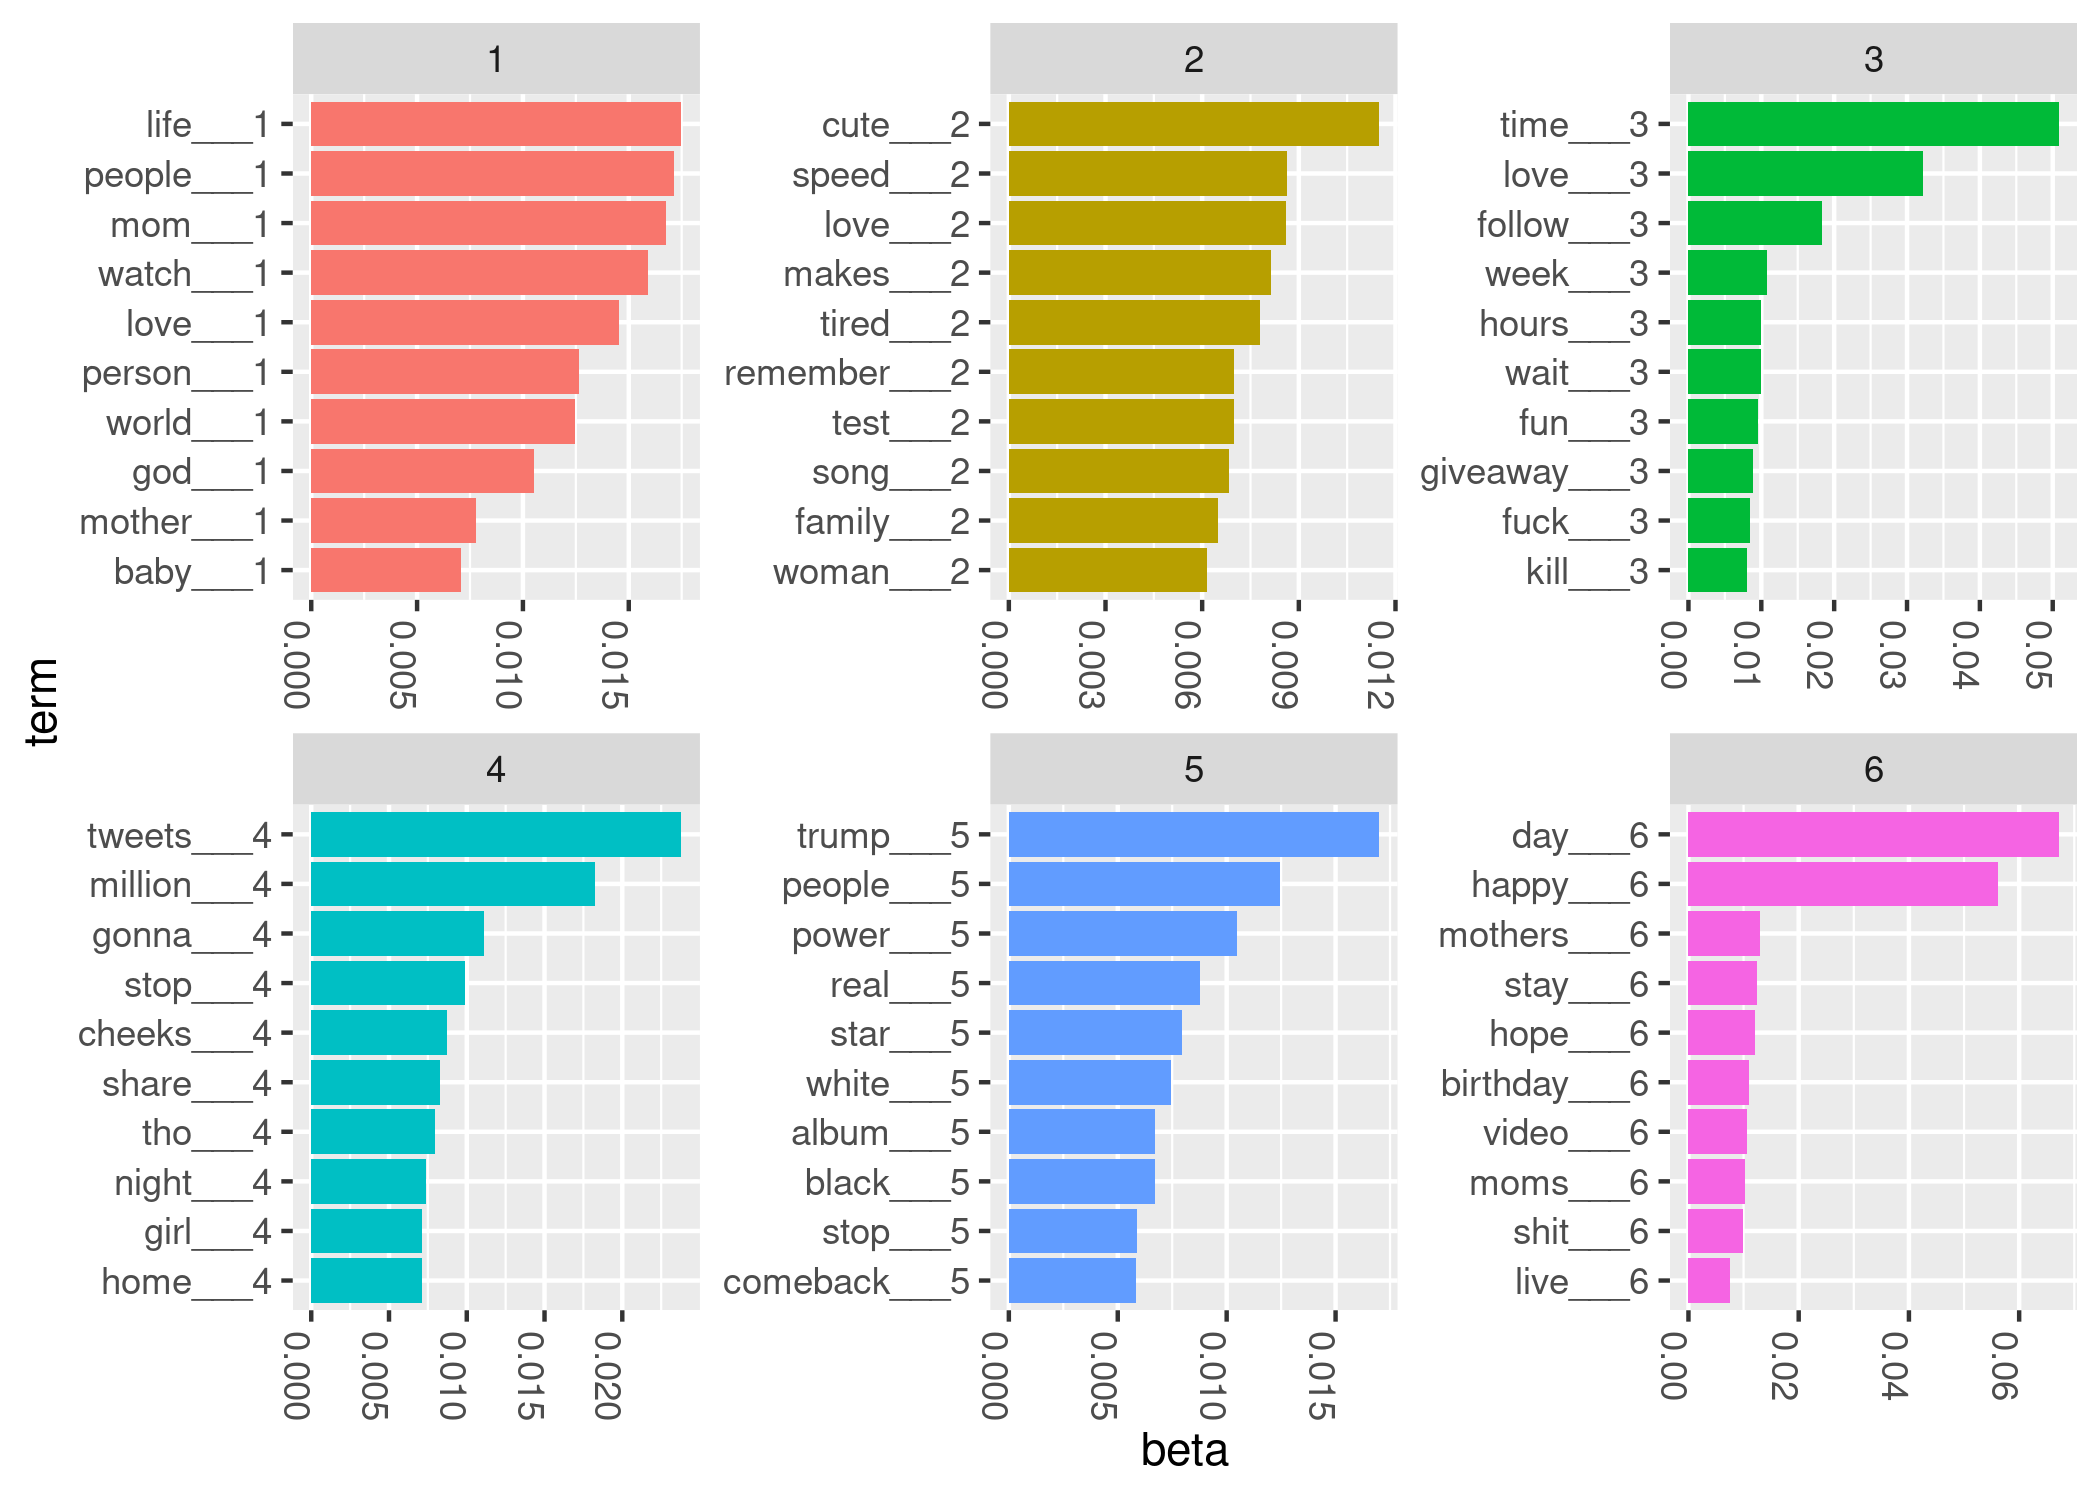
\includegraphics[width=29.17in]{../results/beta-2020-05-10} \caption{Top terms for LDA model from May 10, 2020 (Mother's Day)}\label{fig:unnamed-chunk-5}
\end{figure}

\begin{Shaded}
\begin{Highlighting}[]
\NormalTok{knitr}\OperatorTok{::}\KeywordTok{include_graphics}\NormalTok{(}\StringTok{"../results/beta-2020-05-11.png"}\NormalTok{)}
\end{Highlighting}
\end{Shaded}

\begin{figure}
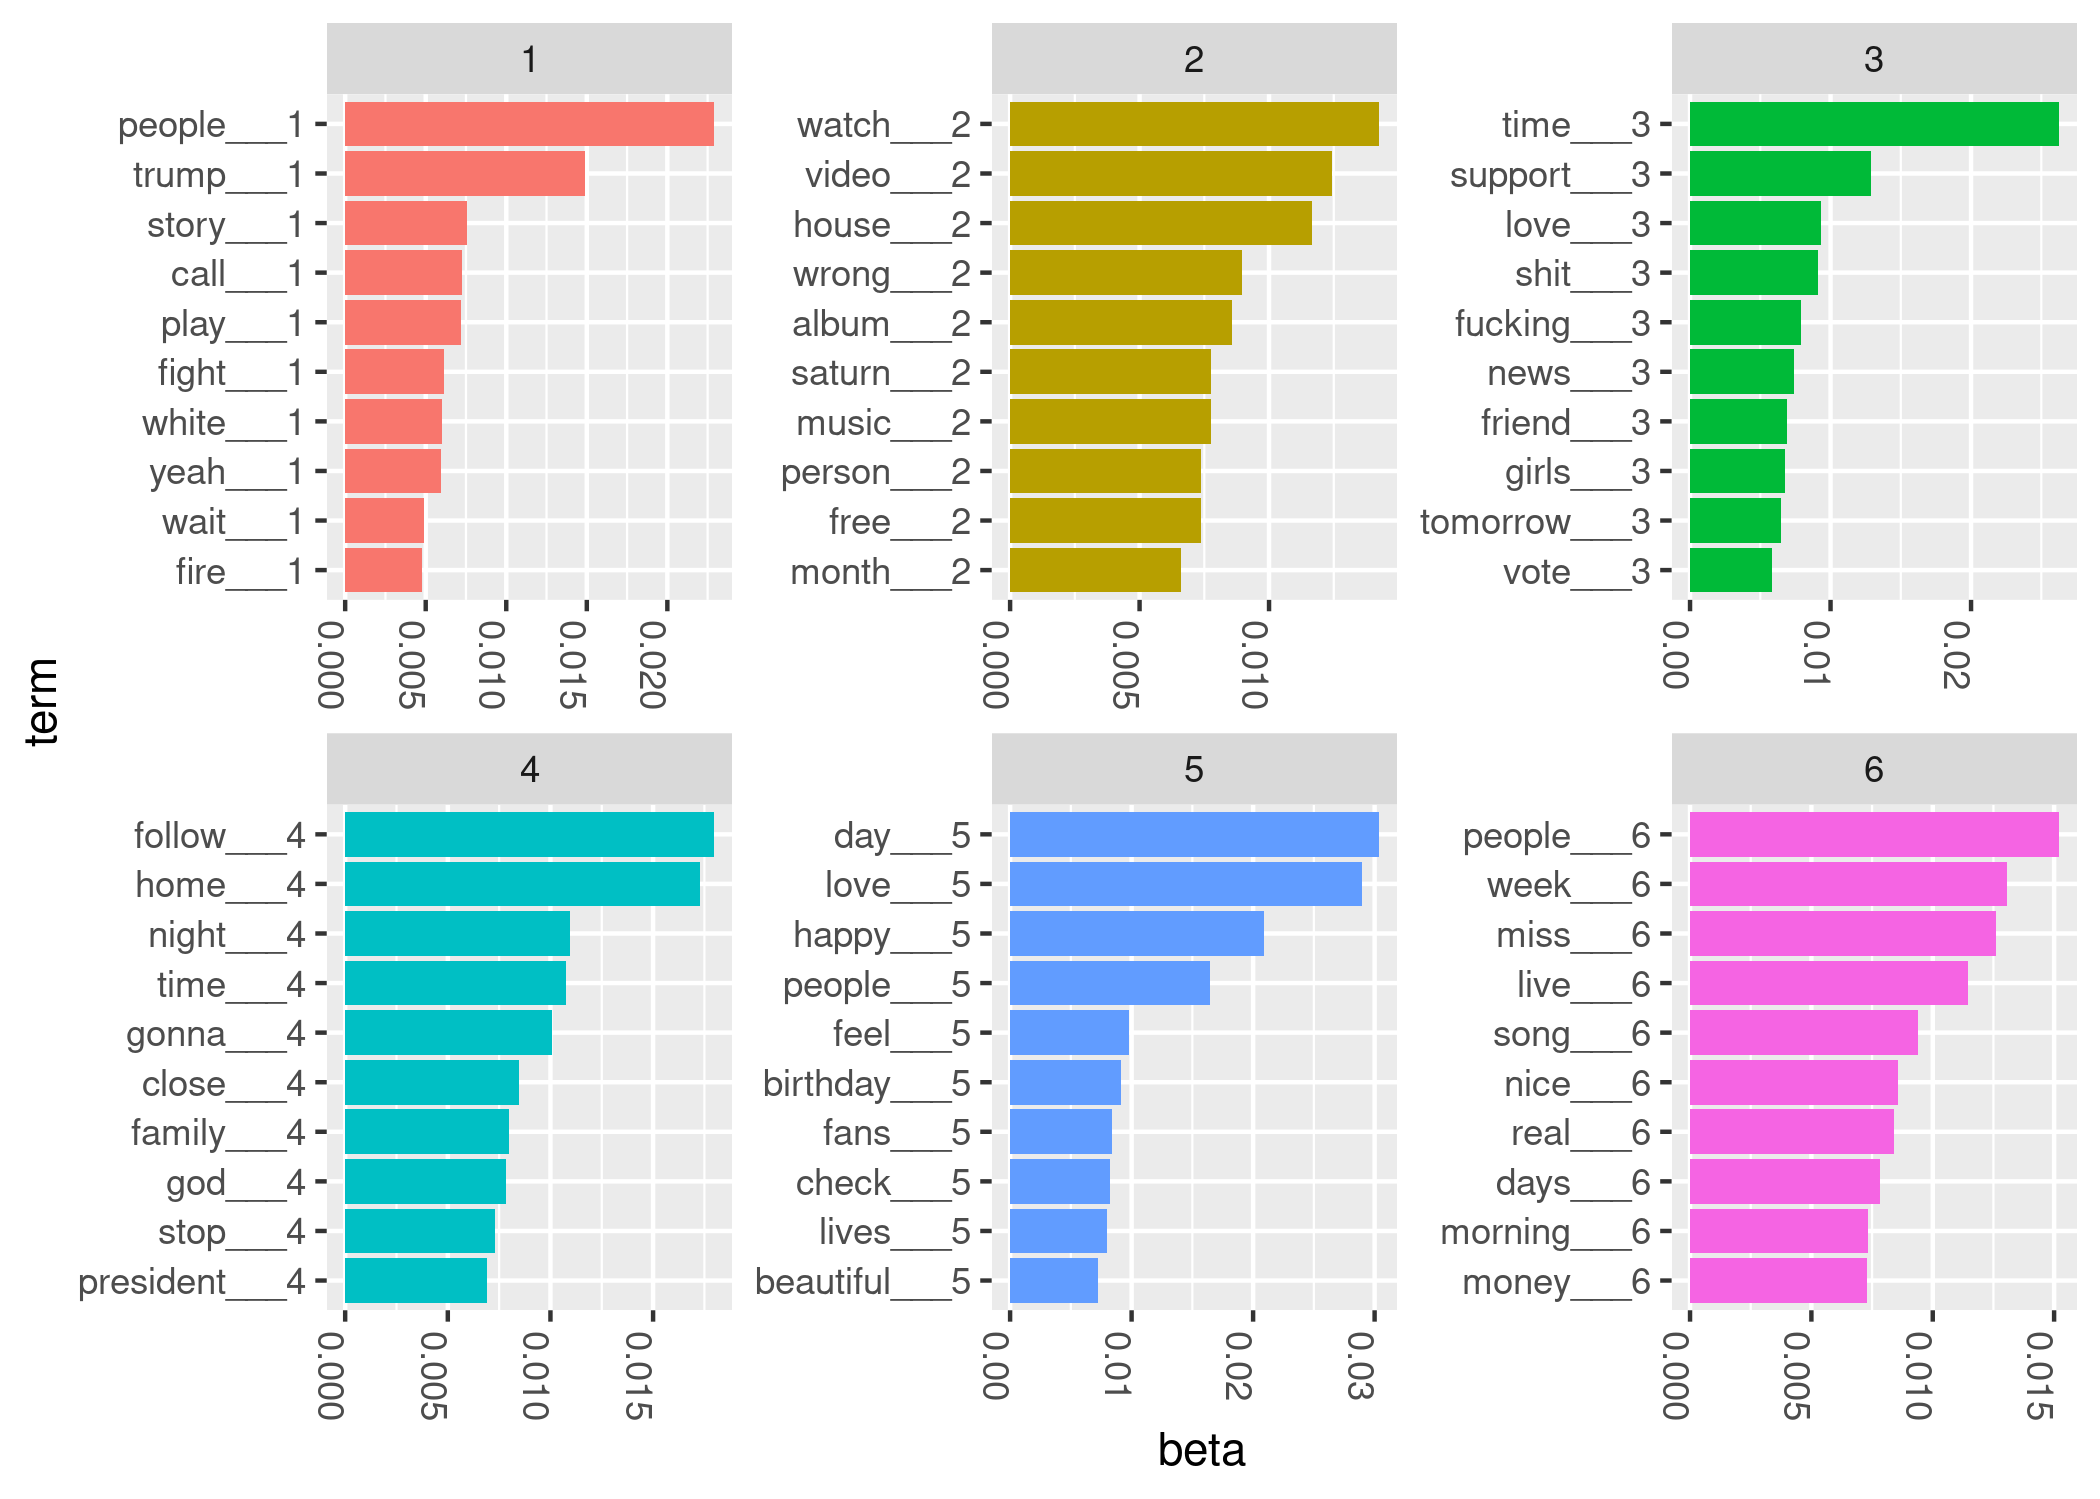
\includegraphics[width=29.17in]{../results/beta-2020-05-11} \caption{Top terms for LDA model from May 11, 2020}\label{fig:unnamed-chunk-6}
\end{figure}

\hypertarget{references}{%
\subsection{References}\label{references}}

\hypertarget{refs}{}
\leavevmode\hypertarget{ref-tweet_json}{}%
``Introduction to Tweet Json.''
\url{https://developer.twitter.com/en/docs/tweets/data-dictionary/overview/intro-to-tweet-json},
2020\\
Accessed: 2020-05-18.

\leavevmode\hypertarget{ref-lin2011joint}{}%
Lin, Cindy Xide, Qiaozhu Mei, Jiawei Han, Yunliang Jiang, and Marina
Danilevsky. ``The Joint Inference of Topic Diffusion and Evolution in
Social Communities.'' In \emph{2011 Ieee 11th International Conference
on Data Mining}, 378--87. IEEE, 2011.

\leavevmode\hypertarget{ref-nolan2010computing}{}%
Nolan, Deborah, and Duncan Temple Lang. ``Computing in the Statistics
Curricula.'' \emph{The American Statistician} 64, no. 2 (2010): 97--107.

\leavevmode\hypertarget{ref-pelled2018little}{}%
Pelled, Ayellet, Josephine Lukito, Fred Boehm, JungHwan Yang, and Dhavan
Shah. ```Little Marco,'`Lyin'Ted,'`Crooked Hillary,' and the `Biased'
Media: How Trump Used Twitter to Attack and Organize.'' In \emph{Digital
Discussions}, 176--96. Routledge, 2018.

\leavevmode\hypertarget{ref-drob}{}%
Robinson, David. ``Text Analysis of Trump's Tweets Confirms He Writes
Only the (Angrier) Android Half.''
\url{http://varianceexplained.org/r/trump-tweets/}, 2016\\
Accessed: 2019-11-26.

\leavevmode\hypertarget{ref-tweet_stream}{}%
``Sampled Stream.''
\url{https://developer.twitter.com/en/docs/labs/sampled-stream/overview},
2019\\
Accessed: 2019-11-27.

\leavevmode\hypertarget{ref-wells2016trump}{}%
Wells, Chris, Dhavan V Shah, Jon C Pevehouse, JungHwan Yang, Ayellet
Pelled, Frederick Boehm, Josephine Lukito, Shreenita Ghosh, and Jessica
L Schmidt. ``How Trump Drove Coverage to the Nomination: Hybrid Media
Campaigning.'' \emph{Political Communication} 33, no. 4 (2016): 669--76.

\newpage

\hypertarget{appendix-1-tweet-data-dictionary}{%
\subsection{Appendix 1: Tweet data
dictionary}\label{appendix-1-tweet-data-dictionary}}

Twitter shares a data dictionary for tweets
(\url{https://developer.twitter.com/en/docs/tweets/data-dictionary/overview/tweet-object},
(Accessed: May 23, 2020)). We have saved it as a supplementary file,
``tweets-data-dictionary.csv''.

\end{document}
